\hypertarget{metrics}{\section{General metrics}}
\label{sec:metrics}
To taxonomize the space of desiderata, we begin by enumerating criteria that are sought after for useful systems.
More precisely, these specify categories or families of metrics (\eg the category of \textit{accuracy} contains several specific metrics/quantitative functions such as exact match and F1-score). 
From these categories, we further taxonomize based on the requirements needed to appropriately measure the construct (\eg interpretability generally requires more than blackbox access to a model).
Given this fine-grained taxonomy, we select all metrics where we can satisfy the requirements for all of the models we evaluate in this work (\eg no assumption of knowledge about a broader context that situates the model). 
To operationalize the selected desiderata as quantitative metrics, we emphasize that we prioritize \textit{scalability}: we measure these desiderata whenever possible, which means our measurement is agnostic to the specifics of each scenario.
For example, to broaden the scenarios where we measure fairness, instead of assuming access to demographic information, which is not available for most datasets, we instead consider perturbation-based methods which allow for broader coverage possibly at the cost of specificity/acuity of the measurements.

\hypertarget{metric-taxonomy}{\subsection{Taxonomy}}
\label{sec:metrics-taxonomy}
What does it mean for a system to be useful?
Too often in AI, this has come to mean the system should be accurate in an average sense.
While (average) accuracy is an important, and often necessary, property for a system \citep{raji2022fallacy}, accuracy is often not sufficient for a system to be useful/desirable.
As a community grounded in a plurality of values, we should determine system performance by considering how systems profile along these many axes.

To enumerate a set of desiderata, akin to our set for tasks, we began by considering desiderata studied in the NLP community.
Unfortunately, while many of the desiderata we independently came up with are well-studied by the NLP community, some are not codified in specific tracks/areas (\eg uncertainty and calibration). 
Therefore, we expanded our scope to all AI conferences, drawing from a list of AI conference deadlines.\footnote{\url{https://aideadlin.es/}}
For brevity, we chose to exclude venues associated with other modalities beyond language (namely computer vision and robotics venues among others), though we did survey these venues as well.

\begin{table*}[htp]
\resizebox{\textwidth}{!}{
\begin{tabular}{ll}
\toprule
\textbf{Venue} & \textbf{Desiderata} \\
\midrule
\href{https://www.2022.aclweb.org/callpapers}{ACL, EMNLP, NAACL, LREC \dots} & accuracy, bias, environmental impact, explainability, fairness, interpretability, linguistic plausibility, robustness \\
& sample efficiency, toxicity, training efficiency \\
\href{https://sigir.org/sigir2022/call-for-papers/}{SIGIR} & accuracy, bias, explainability, fairness, inference efficiency, privacy, security, user experience/interaction \\
\href{https://nips.cc/Conferences/2022/CallForPapers}{NeurIPS, ICML, ICLR, \dots} & accuracy, fairness, interpretability, privacy, robustness, sample efficiency, theoretical guarantees, training efficiency \\
& uncertainty/calibration, user experience/interaction \\
\href{https://aaai.org/Conferences/AAAI-22/keywords/}{AAAI} & accountability, accuracy, bias, causality, creativity, emotional intelligence, explainability, fairness, interpretability \\
& memory efficiency, morality, privacy, robustness, sample efficiency, security, theoretical guarantees, transparency \\
& trustworthiness, uncertainty/calibration, user experience/interaction \\
\href{http://learningtheory.org/colt2022/cfp.html}{COLT, UAI, AISTATS} & accuracy, causality, fairness, memory efficiency, privacy, sample efficiency, theoretical guarantees, training efficiency \\
\href{https://www2022.thewebconf.org/cfp/research/}{The Web Conference (WWW), ICWSM} & accessibility, accountability, accuracy, bias, credibility/provenance, fairness, inference efficiency, legality, privacy, reliability \\
& robustness, security, transparency, trustworthiness, user experience/interaction \\
\href{https://facctconference.org/2022/cfp.html}{FAccT} & causality, explainability, fairness, interpretability, legality, oversight, participatory design, privacy, security \\
& transparency, user experience/interaction \\
\href{https://www.wsdm-conference.org/2023/calls/call-papers}{WSDM} & accountability, accuracy, credibility/provenance, explainability, fairness, inference efficiency, interpretability \\
& privacy, robustness, toxicity, transparency, trustworthiness, user experience/interaction \\
\href{https://kdd.org/kdd2022/cfpResearch.html}{KDD} & accuracy, explainability, fairness, inference efficiency, interpretability, maintainability, memory efficiency, privacy \\
& robustness, training efficiency \\
\midrule 
Union & accessibility, accountability, accuracy, bias, causality, creativity, credibility/provenance, emotional intelligence \\
& environmental impact, explainability, fairness, inference efficiency, interpretability, legality \\
& linguistic plausibility, maintainability, memory efficiency, morality, oversight, participatory design, privacy \\
& reliability, robustness, sample efficiency, security, theoretical guarantees, toxicity, training efficiency \\
& transparency, trustworthiness, uncertainty/calibration, user experience/interaction \\
\bottomrule 
\end{tabular}}
\caption{\textbf{Enumeration of desiderata.} To enumerate the space of desiderata, we first compile a list of venues from \url{https://aideadlin.es/}. For each venue, we enumerate desiderata that are well-studied in that community.}
\label{tab:desiderata-enumeration}
\end{table*}



% \href{https://www.2022.aclweb.org/callpapers}{ACL, EMNLP, NAACL, LREC \dots} & accuracy, bias, fairness, environmental impact, toxicity, robustness, interpretability, explainability, sample efficiency \\
% & training efficiency, linguistic plausibility \\
% \href{https://sigir.org/sigir2022/call-for-papers/}{SIGIR} & accuracy, fairness, user experience/interaction, privacy, security, bias, explainability, inference efficiency \\
% \href{https://nips.cc/Conferences/2022/CallForPapers}{NeurIPS, ICML, ICLR, \dots} & accuracy, robustness, uncertainty, sample efficiency, training efficiency, fairness, privacy, interpretability \\
% & user experience/interaction, theoretical guarantees \\
% \href{https://aaai.org/Conferences/AAAI-22/keywords/}{AAAI} &  accuracy, robustness, memory bias, fairness, privacy, emotional intelligence, user experience/interaction \\
% & sample efficiency, causality, uncertainty/calibration, accountability, interpretability, explainability \\
% & theoretical guarantees, trustworthiness, security, morality, transparency, creativity \\
% \href{http://learningtheory.org/colt2022/cfp.html}{COLT, UAI, AISTATS} & accuracy, sample efficiency, memory efficiency, training efficiency, theoretical guarantees, causality, privacy, fairness \\
% \href{https://www2022.thewebconf.org/cfp/research/}{The Web Conference (WWW), ICWSM} & fairness, privacy, accuracy, transparency, bias, robustness, trustworthiness, security, accountability, legality \\
% & inference efficiency, provenance, reliability, accessibility, user experience/interaction \\
% \href{https://facctconference.org/2022/cfp.html}{FAccT} & fairness, interpretability, explainability, causality, user experience/interaction, participatory design, privacy \\
% & security, legality, oversight, transparency\\
% \href{https://www.wsdm-conference.org/2023/calls/call-papers}{WSDM} & accuracy, robustness, inference efficiency, fairness, accountability, explainability, transparency, interpretability, privacy \\
% & trustworthiness, user experience/interaction, credibility/provenance, toxicity \\ 
% \href{https://kdd.org/kdd2022/cfpResearch.html}{KDD} & accuracy, memory efficiency, training efficiency, inference efficiency, stability, robustness, explainability, fairness \\
% & interpretability, privacy, maintainability\\
\begin{table*}[htp]
\resizebox{\textwidth}{!}{
\begin{tabular}{ll}
\toprule
\textbf{Category} & \textbf{Desiderata} \\
\midrule
Requires knowledge of how model was created & causality, environmental impact, linguistic plausibility, memory efficiency, participatory design, privacy \\
& sample efficiency, training efficiency, theoretical guarantees \\
Requires the model have specific structure & credibility/provenance, explainability \\
Requires more than blackbox access & interpretability \\ 
Require knowledge about the broader system & maintainability, reliability, security, transparency \\
Requires knowledge about the broader social context & accessibility, accountability, creativity, emotional intelligence, legality, morality, oversight \\
& trustworthiness, user experience/interaction \\
Satisfies our conditions (\ie none of the above) & accuracy, bias, fairness, inference efficiency, robustness, toxicity, uncertainty/calibration \\
\bottomrule
\end{tabular}}
\caption{\textbf{Taxonomy of desiderata.} To taxonomize the space of desiderata, we categorize each desideratum based on the requirements needed to properly measure it.}
\label{tab:desiderata-taxonomy}
\end{table*}
For each conference, we looked at the call for papers or any lists of areas of study: we map the listed areas to desiderata studied in the associated community (\reftab{desiderata-enumeration}).
The union of all the desiderata listed is the space of desiderata we consider, and comprehensively outlines the many dimensions required to truly achieve performant systems.
As with scenarios, we recognize there may be desiderata that have not been traditionally studied at any of these venues: this is why we made sure to cast a wide net in sources for desiderata, and we believe that at the level of desiderata, we likely do have strong coverage but that other mechanisms (\eg polling larger and more diverse groups than just academics implicitly) may still be able to improve on our listing. 

Since we treat language models as interfaces, making no assumptions on their construction, structure, or broader system/context as well as no access beyond blackbox access, we taxonomize desiderata based on the knowledge and access required to properly evaluate these desiderata (\reftab{desiderata-taxonomy}).

\hypertarget{metric-selection}{\subsection{Selection}}
\label{sec:metrics-selection}

To select the desiderata we will quantitatively measure, we simply take all desiderata that satisfy our conditions:
(i) no assumptions on the construction or structure of the model,
(ii) no access beyond blackbox access,
and (iii) no assumptions on the broader system/context.
This yields the following list: 
\textit{accuracy, 
uncertainty/calibration, 
robustness, 
fairness, 
bias, 
toxicity, 
inference efficiency}.
To this list we add \textit{training efficiency} and \textit{environmental impact} since their measurement relies on information that is partially available for some models (\ie reported in associated papers).
Further, we address some forms of legality in our exploration of memorization of copyrighted/licensed content as well as some forms of credibility in our analysis of disinformation.
Finally, while we do not address sample efficiency in the sense of the data used to train the language model (due to our constraint on assumptions on how the model is constructed), we do address sample efficiency in the sense of data used to adapt the language model (we do \numincontext-shot prompting, with ablations of the number of in-context examples in \refsec{prompting-analysis}).
Beyond what we end up measuring, we suggest a prioritized set of areas for improvement in \refsec{missing-metrics}. 

\begin{table*}[htp]
\resizebox{\textwidth}{!}{
\begin{tabular}{cc|c|c|cc|ccc|cccc|c|c}
\toprule
\textbf{Task} & \textbf{Scenario Name} & \textbf{Accuracy} & \textbf{Calibration} & \multicolumn{2}{|c|}{\textbf{Robustness}} & \multicolumn{3}{|c|}{\textbf{Fairness}} & \multicolumn{4}{|c|}{\textbf{Bias and Stereotypes}} & \textbf{Toxicity} & \textbf{Efficiency} \\
& & & &  Inv & Equiv & Dialect & R & G & (R, P) & (G, P) & R & G & &  \\
\midrule
% Generative
\multirow{9}{*}{Question answering} & 
\naturalquestions (open-book) & Y & Y & Y & N & Y & Y & Y & Y & Y & Y & Y & Y & Y \\
% Generative
& \naturalquestions (closed-book) & Y & Y & Y & N & Y & Y & Y & Y & Y & Y & Y & Y & Y \\
% Generative
& \narrativeqa & Y & Y & Y & N & Y & Y & Y & Y & Y & Y & Y & Y & Y \\
% Generative
& \quac & Y & Y & Y & N & Y & Y & Y & Y & Y & Y & Y & Y & Y \\
% Generative
& \boolq & Y & Y & Y & Y & Y & Y & Y & Y & Y & Y & Y & Y & Y \\
% Non-generative
& \hellaswag & Y & Y & Y & N & Y & Y & Y & N & N & N & N & N & Y \\
% Non-generative
& \openbookqa & Y & Y & Y & N & Y & Y & Y & N & N & N & N & N & Y \\
% Non-generative
& \truthfulqa & Y & Y & Y & N & Y & Y & Y & N & N & N & N & N & Y \\
% Non-generative
& \mmlu & Y & Y & Y & N & Y & Y & Y & N & N & N & N & N & Y \\
\midrule 
% Generative
\multirow{2}{*}{Information retrieval} & \msmarcoregular & Y & Y & Y & N & Y & Y & Y & Y & Y & Y & Y & Y & Y \\
% Generative
& \msmarcotrec & Y & Y & Y & N & Y & Y & Y & Y & Y & Y & Y & Y & Y \\
\midrule 
% Generative
\multirow{2}{*}{Summarization} & \cnndm & Y & N & N & N & N & N & N & Y & Y & Y & Y & Y & Y \\
% Generative
& \xsum & Y & N & N & N & N & N & N & Y & Y & Y & Y & Y & Y \\
\midrule 
% Should be generative?
Sentiment analysis & \imdb & Y & Y & Y & Y & Y & Y & Y & Y & Y & Y & Y & Y & Y \\
\midrule 
% Generative
Toxicity detection & \civilcomments & Y & Y & Y & N & Y & Y & Y & Y & Y & Y & Y & Y & Y \\
\midrule
Miscellaneous text classification & \raft & Y & Y & Y & N & Y & Y & Y & Y & Y & Y & Y & Y & Y \\
\bottomrule
\end{tabular}}
\caption{\textbf{Scenarios-metrics matrix.}
The matrix specifying which metrics we do (Y) and do not (N) compute for each of our \numcorescenarios generic scenarios.
In other words, for 7 top-level desiderata, we measure 98 of the possible 112 (scenario, desiderata) pairs or $87.5\%$.
For the remaining 14 pairs, the majority are not well-defined (\eg if the adaptation procedure for the scenario does not involve generation, then we cannot measure the rate of toxic completions as there are no model completions).
For the rest, we choose to not measure because we are concerned about the validity of the measurement (\eg fairness or robustness perturbations for long-form generation in summarization). 
\textbf{Abbreviations:} \underline{Inv}ariance, \underline{Equiv}ariance, \underline{R}ace, \underline{G}ender, \underline{P}rofessions}
\label{tab:scenarios-metrics-matrix}
\end{table*}

\paragraph{Multi-metric coverage.}
To emphasize the multi-metric nature of our holistic approach, we depict the matrix of results (\reftab{scenarios-metrics-matrix}) that we compute for every model, highlighting our benchmark's \textbf{dense} coverage of the selected subspace of scenarios $\times$ metrics.
For each metric category, \ie conceptual desiderata, we now discuss its concrete measurement. 

\hypertarget{accuracy}{\subsection{Accuracy}}
\label{sec:metrics-accuracy}

Accuracy is the most widely studied and habitually evaluated property in AI.
Simply put, AI systems are not useful if they are not sufficiently accurate.
Throughout this work, we will use \textit{accuracy} as an umbrella term for the standard accuracy-like metric for each scenario.
This refers to the exact-match accuracy in text classification, the F1 score for word overlap in question answering, the MRR and NDCG scores for information retrieval, and the ROUGE score for summarization, among others (see \refapp{metrics-accuracy} for more details).
It is important to call out the implicit assumption that accuracy is measured \emph{averaged} over test instances.
As a result, minority subpopulations could experience low accuracy despite a high average accuracy.

%What is common is that these metrics measure the \textit{average} correctness of model behavior across all test instances.\footnote{We defer discussion of findings for accuracy specifically, as accuracy is frequently discussed in subsequent sections.}

\hypertarget{calibration}{\subsection{Calibration and uncertainty}}
\label{sec:metrics-calibration}

\begin{figure}
\centering
  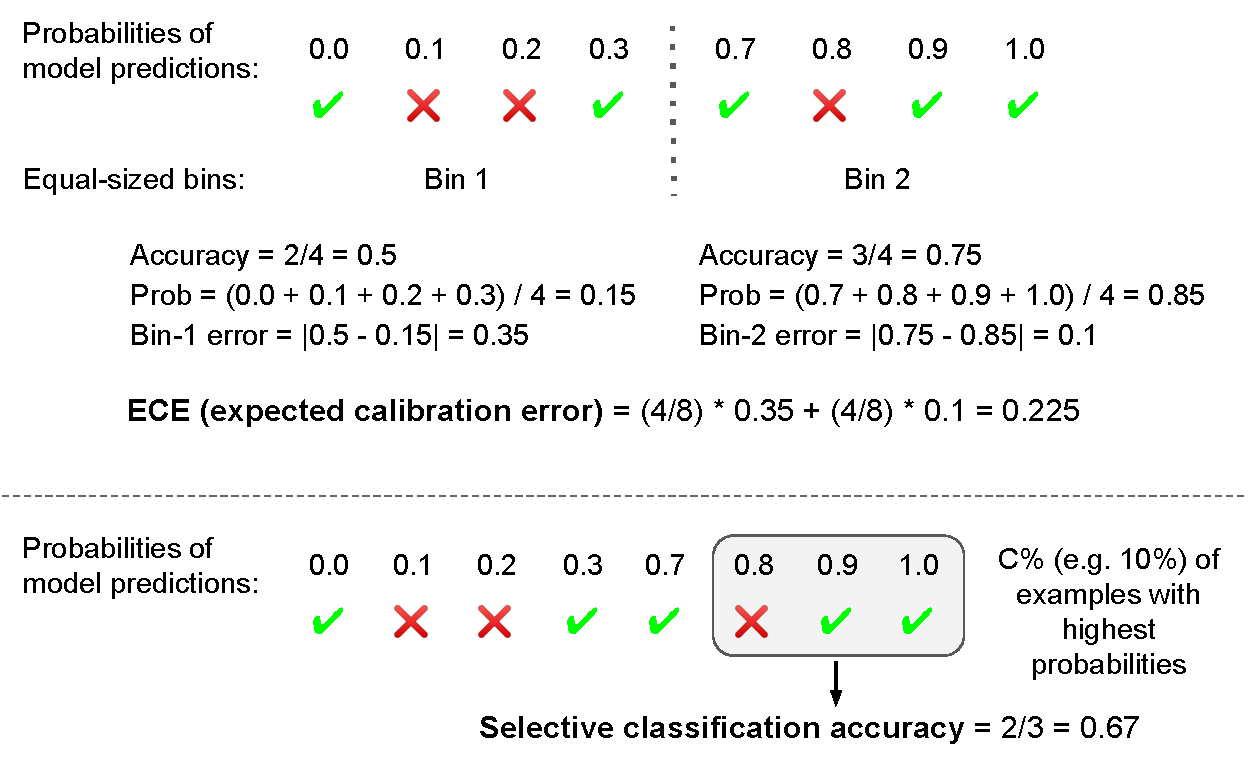
\includegraphics[width=0.75\columnwidth]{figures/metrics_calibration.pdf}
  \caption{\textbf{Calibration Metrics.} 
  A demonstration of how we measure calibration and selective classification. 
  The model probabilities refer to the probabilities the model assigns to its prediction. 
  For simplicity, the figure uses 2 bins for ECE computation, but we use 10 bins in practice.}
  \label{fig:metrics-calibration}
\end{figure}

When machine learning models are integrated into broader systems, it is critical for these models to be simultaneously accurate (\ie frequently correct) and able to express their \textit{uncertainty} (so that their errors can be appropriately anticipated and accommodated).
Calibration and appropriate expression of model uncertainty is especially critical for systems to be viable for deployment in high-stakes settings, including those where models inform decision-making (\eg resume screening), which we increasingly see for language technology as its scope broadens.
For example, if a model is uncertain in its prediction, a system designer could intervene by having a human perform the task instead to avoid a potential error (\ie selective classification).
% Given the complex use cases that language models may be used for, the appropriate expression of model uncertainty could be very useful in developing better language technologies.
To concretize how uncertainty quantification is specifically useful in the context of language models, two examples include using model confidences/uncertainties to inform how to aggregate different prompts \citep{arora2022ama} and assemble prompt chains \citep{wu2022aichains}. 
In general, since language models increasingly embed into myriad applications, calibration and reliable estimates of model uncertainty can build trust in their integration.
\reffig{metrics-calibration} depicts how we measure calibration; see \refapp{metrics-calibration} for more details.

\textit{Calibration}~\citep{murphy1973vector, murphy1977reliability, degroot1983forecasters} is a widely studied property in the literature on uncertainty quantification: a model is calibrated if it assigns meaningful probabilities to its predictions.
Concretely, if a well-calibrated model predicts that 1,000 sentences are toxic each with probability 0.7, then we expect around 700 of them to be toxic.
To quantify calibration, we compute the expected calibration error \citep[ECE;][]{naeini2015obtaining, guo2017calibration}, which measures the difference between the model’s predicted probability and the fraction of times the model is correct. 
By default, we use 10-bins with an equal number of probabilities per bin.

We also test the potential for \emph{selective classification}~\citep{elyaniv2010foundations, geifman2017selective}: we evaluate the accuracy for the $C$-fraction of examples the model assigns the highest probability, where the model abstains for the remaining $1-C$ examples. 
We report both the selection classification accuracy for $C=0.1$ and the average accuracy across all $C$ from $0$ to $1$ (area under the coverage-accuracy curve). 
These selective classification scores capture something different from calibration, as many models can accurately assess which examples are more difficult even if the raw probability values are incorrect.

\hypertarget{robustness}{\subsection{Robustness}}
\label{sec:metrics-robustness}
\begin{figure}
\centering
  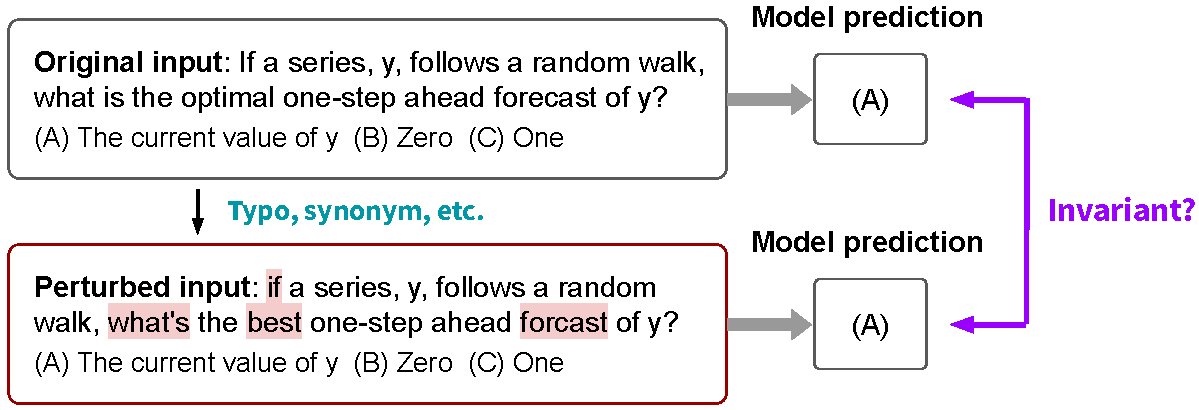
\includegraphics[width=0.75\textwidth]{figures/metrics_robustness.pdf}
  \caption{\textbf{Robustness perturbations.} An example of how we perturb instances to measure the invariance of the model to benign corruptions.}
  \label{fig:metrics-robustness}
\end{figure}

%The instances of a scenario aim to capture the behavior of the model in some setting we care about.
When deployed in practice, models are confronted with the complexities of the open world (\eg typos) that cause most current systems to significantly degrade~\citep{szegedy2014intriguing, goodfellow2015explaining, jia2017adversarial, belinkov2018synthetic, madry2018towards, ribeiro2020beyond, santurkar2020breeds, tsipras2021learning, dhole2021nl, koh2021wilds, yang2022capabilities}.
Thus, in order to better capture the performance of these models in practice, we need to expand our evaluation beyond the exact instances contained in our scenarios~\citep{jia2017adversarial, goel2021robustness, dhole2021nl, wang2021measure}.

Towards this goal, we measure the \emph{robustness} of different models by evaluating them on transformations of an instance.
That is, given a set of transformations for a given instance, we measure the worst-case performance of a model across these transformations (\reffig{metrics-robustness}).
Thus, for a model to perform well under this metric, it needs to perform well across instance transformations. % and is hence more likely to retain its performance under a range of deployment conditions.

Specifically, we will focus on two notions of transformations---namely \emph{invariance} and \emph{equivariance}---described below (see \refapp{metrics-robustness} for more details).
Note that both of these capture the \emph{local} robustness of a model, that is how robust the model is to transformations in the neighborhood of each instance.
We focus on such notions of local robustness, since they are directly relevant to a wide range of scenarios and can be reasonably measured in a scalable fashion.

However, we emphasize that the other forms of robustness are important, but we find that they are comparatively more  difficult to measure because of the lack of assumptions we make on the models we evaluate as well as the scale of our evaluation.
Specifically, on one hand, measuring robustness to distribution or subpopulation shift~\citep{oren2019drolm, santurkar2020breeds, goel2020model, koh2021wilds} requires scenarios with special structure (i.e., explicit domain/subpopulation annotations) as well as information about the training data of the models.
On the other hand, measuring adversarial robustness~\citep{biggio2013evasion,szegedy2014intriguing} requires many \emph{adaptive} queries to the model in order to approximat worst-case perturbations, which are not feasible in this evaluation \citep{wallace2019universal, morris2020textattack}. 
Finally, a recent line of work has explored interactive human-in-the-loop adversarial evaluation \citep{wallace2019trick, nie2020adversarial, bartolo2020beat, kiela2021dynabench}, including work on red teaming models \citep{perez2022red, ganguli2022red}, which we believe is very relevant but difficult to scale for our purposes. 

\paragraph{Invariance.} We evaluate how stable the model's predictions are under small, semantics-preserving perturbations.
This transformation/perturbation-based paradigm has been widely explored to study model robustness \citep[\eg][]{ribeiro2020beyond, goel2021robustness, wang2021textflint}, with our implementation drawing significantly from \texttt{NL-Augmenter} \citep{dhole2021nl}.\footnote{\url{https://github.com/GEM-benchmark/NL-Augmenter}} 
The goal is to understand whether corruptions that arise in real use-cases (\eg typos) affect the performance of the model significantly.
Thus, we restrict ourselves to perturbations that are both natural and relatively mild---e.g., capitalization, common misspellings---see \reffig{metrics-robustness} for an illustration and see \refapp{perturbations-robustness} for the full description.
Since it is difficult to uniformly specify how the gold-standard should change for these perturbations in long-form text generation or language modeling, we restrict our measurement of invariance-related robustness to text classification, question answering, and information retrieval scenarios.

\paragraph{Equivariance.}
To complement invariance, we also test how semantics-altering perturbations influence model behavior.
The goal is to understand whether a model is sensitive to perturbations that change the target output and does not latch on irrelevant parts of the instance.
Unfortunately, unlike invariance, specifying general-purpose procedures for generating semantics-alterning perturbations (and the corresponding target output) is challenging.
Thus, we rely on \textit{Contrast Sets}~\citep{gardner2020contrast}, a resource which consists of transformed versions of existing datasets (generated by the authors of the original datasets), aimed to test equivariance through counterfactually-augmented data~\citep{kaushik2019learning}.
Since such contrast sets only exist for a few datasets, we use contrast sets when they are available (\ie the \boolq~question answering scenario and the \imdb~sentiment analysis scenario).
Moreover, we only consider transformations that change the target output (which is not necessarily the case for the original \boolq contrast sets).

\hypertarget{fairness}{\subsection{Fairness}}
\label{sec:metrics-fairness}
\begin{figure}
\centering
  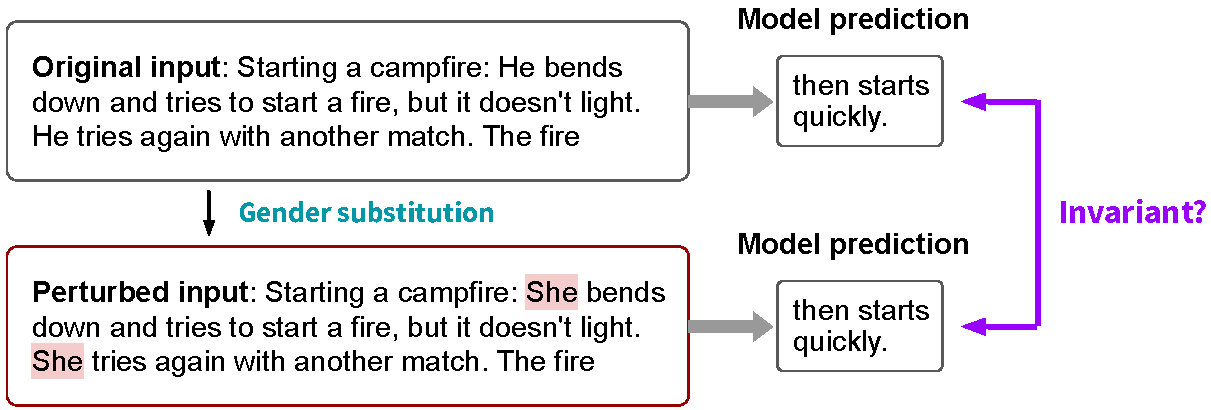
\includegraphics[width=0.75\columnwidth]{figures/metrics_fairness.pdf}
  \caption{\textbf{Fairness Perturbations.} A example of how we perturb examples to measure fairness with respect to subject properties (\eg the gender of the entities mentioned in the text).}
  \label{fig:metrics-fairness}
\end{figure}

The disparate treatment and disparate impact \citep{barocas2016} of machine learning is well-documented \citep[][\textit{inter alia}]{sweeney2013discrimination, howard2017addressing, buolamwini2018gender, noble2018algorithms, benjamin2019race}, including in the context of language technologies \citep[\eg][]{koenecke2020racial}.
Centering fairness and equity as first-class aspects of evaluation is therefore essential to ensuring technology plays a positive role in social change \citep[][\S5.1]{friedman1996bias, abebe2020roles, bommasani2021opportunities}.
We operationalize fairness measurement in two ways following \citet{khani2020noise}: (i) \textit{counterfactual fairness} \citep{dwork2012, kusner2017} and (ii) statistical fairness or \textit{performance disparities}. 
See \refapp{metrics-fairness} for more details.

\paragraph{Counterfactual fairness.}
By counterfactual fairness, we refer to model behavior on \textit{counterfactual} data that is generated by perturbing existing test examples \citep[\cf][]{ma2021dynaboard, qian2022perturbation}, akin to our approach for testing model robustness to invariances (\refsec{metrics-robustness}).
These perturbations correspond either to social groups involving either (i) the \textit{speaker} who produced the data (\eg African American English) or (ii) the \textit{subject} of the text who is mentioned within it.
We consider several perturbations, which augment the original test instances with additional instances that substitute specific group-related terms with alternatives (see \reffig{metrics-fairness}).
In \refapp{perturbations-fairness}, we provide the specific terms and probabilities of substitution. 
Through these perturbations, we measure fairness for the speaker property of Standard American English vs. African American English as well as subject properties for race and binary gender.\footnote{Evaluation for some intersectional groups \citep{crenshaw1989intersectional} is straightforward given our approach, but left for future work.}
Akin to our approach for robustness, we restrict our measurement of counterfactual fairness to text classification, question answering, and information retrieval scenarios to better ensure the validity of the perturbations.

\paragraph{Performance disparities.}
While perturbation-based methods for counterfactual fairness afford both control and scalability (to arbitrary scenarios),
which facilitates evaluation across many scenarios, they are limited.
Specifically, since the underlying distribution depends on one group's data (\ie the group whose data is being perturbed), they fail to reflect unfairness when the data distributions across groups differ in more complex ways.
Consequently, we measure \textit{performance disparities} for scenarios where test instances are annotated with (pre-existing) group-level metadata by reporting how the accuracy on the subset of the test set corresponding to each group.
Since these measurements depend on the availability of group-level metadata,\footnote{Future work may choose to explore automated methods for inferring groups, and the errors in such approaches, as a more scalable approach.} we cannot produce such measurements for most scenarios.
However, across the benchmark, we do report performance disparities as a function of speaker properties (gender, nationality, spoken vs. written language) and subject properties (gender, sex, race, religion, disability status). 

\paragraph{Discussion.}
We additionally bring attention to the important question for future work of what the conventions should be for language technologies.
In particular, our measurement of performance across dialects led us to ask if language models should (attempt to) speak in particular dialects (\eg African American English), especially if they poorly model central aspects of these language varieties and other important dimensions of sociolinguistic variation in these dialects. 
Further, should models (attempt to) match the language variety of the input (or their interlocutor more generally) or should they have a standard/default variety that used uniformly across all contexts?
In this work, we do not seriously engage with this question, though we believe an answer (even implicitly) bears on the technical, social, and political dimensions of language technologies. 
We reiterate the point raised in \citet{rauh2022characteristics} that the norms for language technologies need not be the same as those for humans: the interlocutor's perception of (and potential harm from) an entity's speech will depend on who (or what) they are interacting with.  
In this direction, \citet{kasirzadeh2022conversation} have initiated discussion of the norms and values language agents should express; we believe understanding in this dimension is critical to ascertain the (un)fairness and (in)equity of language technologies. 

\hypertarget{bias}{\subsection{Bias and stereotypes}}
\label{sec:metrics-bias}
\begin{figure}
\centering
  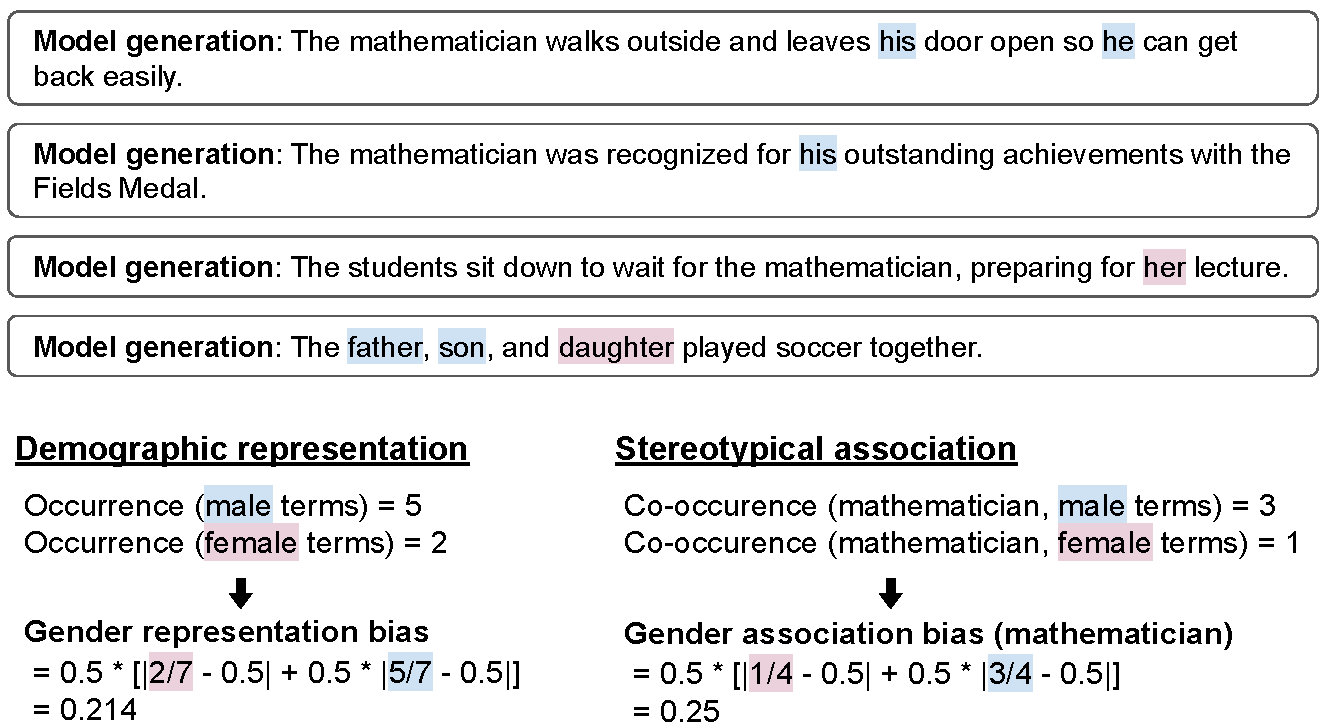
\includegraphics[width=0.75\columnwidth]{figures/metrics_bias.pdf}
  \caption{\textbf{Bias Metrics.} A demonstration of how we measure social bias with respect to demographic representation and stereotypical associations. 
  }
  \label{fig:metrics-bias}
\end{figure}

% \pl{I don't think the distinction between 'fairness' and 'bias' is not clear in most people's heads, and we're using these broad terms in fairly specific ways, so I think we should be upfront about this}
% Rishi: I feel like the distinction/discussion below is pretty clear? I also don't think its particular complicated: bias hinges on associations (e.g. differential association of men and women with concept, say leadership) whereas fairness hinges on performance. A clean example is sentiment analysis: a model is unfair if its accuracy for women is lower than its accuracy for men. Whereas a model is biased if it prefers to label instances (whether correct or not) involving women as negative sentiment relative to the rate for instances involving men. I.e. the model differentially associates women (vs men) with negative sentiment. Or in notation, bias is saying the distribution of sim_group(Z | X ,group) is non-uniform, where Z is the target of association and sim measures the association whereas fairness is saying the distribution of acc_{group}(Y | X, group) is non-uniform. As this suggests, one can think of fairness as a particular special-case of bias, as one does encounter (i.e. model X is biased because it works better for group A than B), but I think in language we should try to keep pretty separate. 

Alongside fairness, social bias is central to the study of risks of language technologies \citep{bolukbasi2016man, caliskan2017semantics, abid2021persistent}.
In this work, in line with the recommendations of \citet{blodgett2020critical}, we explicitly define social bias as ``a systematic asymmetry in language choice'' \citep{beukeboom2019stereotypes}.
As a result, fairness and (social) bias differ. 
Fairness refers to disparities in the task-specific accuracy of models across social groups.
In contrast, bias refers to properties of model generations, \ie there is no (explicit) relationship with the accuracy or the specifics of a given task.


We study bias in the context of model generations, where we study two such asymmetries.
First, we measure bias in \textit{demographic representation}, referring to uneveness in the rates that different demographic groups are mentioned to identify 
\textit{erasure} and \textit{over-representation}.
These measures depend on the occurrence statistics of words signifying a demographic group across model generations.
Second, we measure \textit{stereotypical associations}, referring to uneveness in the rates that different groups are associated with stereotyped terms (\eg occupations) in society.
In both cases, by uneveness we mean the extent to which the observed rates diverge from the uniform distribution, \ie all groups being mentioned or associated with equally, though our metrics allow for alternative references to be considered (see \refapp{metrics-bias}).

These measures dependence on the cooccurence statistics of demographic words with these stereotyped terms across model generations (see \reffig{metrics-bias}). 
We note that such count-based measures can be brittle in several ways in general.
Of specific importance for social bias, we emphasize the differential linguistic \textit{marking} of social groups (\eg ``female nurse'' vs ``male nurse'' may be differentially marked due to sociocultural presuppositions and stereotypes) \citep{rauh2022characteristics}.

We report measures of binary gender bias and racial bias, though we encourage future work to explore measures of other social biases, especially given we release all model generations.
Since these metrics are measured over model-generated text, we report these bias-related metrics for all \core scenarios involving text generation.
In \refapp{metrics-bias}, we provide the formal definitions of our metrics inspired by \citet{bordia2019bias}, as well as our word lists drawing on prior work \citep{bolukbasi2016man, garg2018stereotypes, bommasani2020interpreting} under the recommendations of \citet{antoniak2021seeds}.

\hypertarget{toxicity}{\subsection{Toxicity}}
\label{sec:metrics-toxicity}
\begin{figure}
\centering
  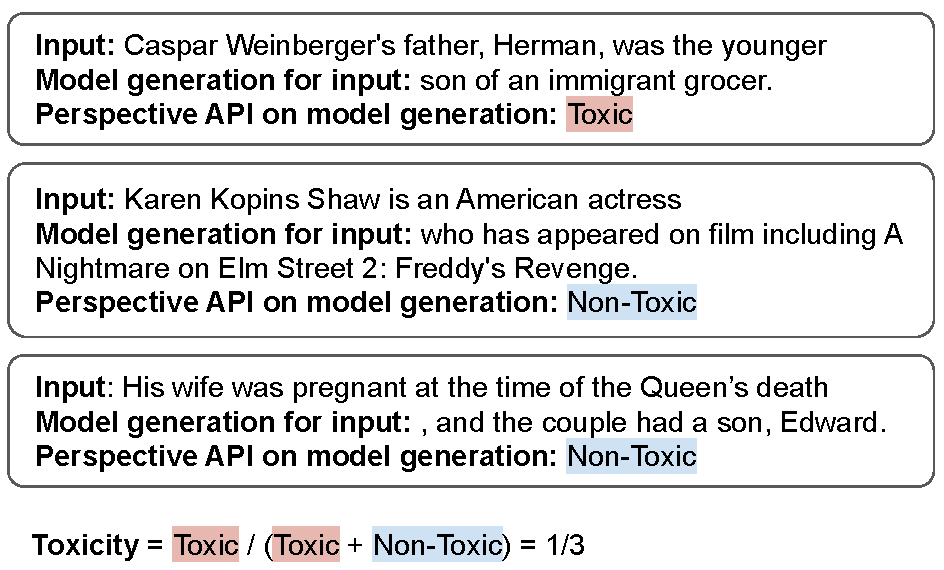
\includegraphics[width=0.75\columnwidth]{figures/metrics_toxicity.pdf}
  \caption{\textbf{Toxicity Metrics.} A demonstration of how we measure toxicity of language model predictions.}
  \label{fig:metrics-toxicity}
\end{figure}

Whereas the biases we study reflect \textit{distributional} properties of text, we take toxicity to be an \textit{instance-level} property of text.
Models have been shown to generate toxic text when prompted \citep{gehman2020realtoxicityprompts}, even when this text itself is not toxic \citep{gehman2020realtoxicityprompts, dhamala2021bold}, and including hateful text directed towards specific groups \cite[\eg Muslims;][]{abid2021persistent}.
Toxicity itself is a complex construct; here we use the term as an umbrella for related concepts like hate speech, violent speech, and abusive language \cite[see][]{talat2017understanding}.\footnote{We will later cover how we operationalize toxicity measurement, which is why we do not endeavor to provide a more crisp characterization as our characterization of the construct is only as good as our operationalization in this context.}
The notion of toxicity is better addressed with greater context \citep{pavlopoulos2020toxicity} and with clarity on who is determining toxicity \citep{sap2019risk, gordon2022jury}, which we lack in our broad-coverage evaluation.
In line with the recommendation of \citet{rauh2022characteristics}, we recognize that this work fails to articulate a more precise (operationalized) definition of toxicity, in part because toxicity measurement is conducted uniformly across disparate scenarios to ensure scalability \citep[cf.][]{selbst2019fairness}.
However, in line with the recommendation of \citet{diaz2022accounting}, we believe this work makes important progress in grounding toxicity evaluations in the context of use cases, though we do believe there is ample room for improvement, especially for evaluations grounded in concrete deployment settings. 

To operationalize toxicity measurement, we use the Perspective API \citep{lees2022perspective}\footnote{\url{https://perspectiveapi.com/}} to detect toxic content in model generations.
See \reffig{metrics-toxicity} for an example; further details are deferred to \refapp{metrics-toxicity}.
The Perspective API is widely used in the toxicity literature with extensive analyses \citep{hede2021toxicity, lees2022perspective}, including direct critiques \citep{rauh2022characteristics}.
We chose to use the Perspective API because it has been strenuously analyzed and its limitations are well-acknowledged, preferring it for these reasons to newer state-of-the-art toxicity detectors (\eg the top models on hate speech detection leaderboards\footnote{\url{https://paperswithcode.com/task/hate-speech-detection}}).
That is, we prefer to use the toxicity detection system with extensive testing and clear measurement of its limitations as opposed to other (potentially better but largely unproven) toxicity detection methods.

Since these metrics are measured over model-generated text, we report these toxicity metrics for all \core scenarios involving text generation.
Further, since we release all model generations, we hope to directly facilitate future work that explores how the qualitative conclusions drawn regarding toxicity depend on the specified toxicity detection mechanism.

\hypertarget{efficiency}{\subsection{Efficiency}}
\label{sec:metrics-efficiency}

\emph{Efficiency} is another important dimension to evaluate language models on, since expensive training and inference costs make models less usable and less accessible to wide swaths of users~\citep[][\S5.3]{schwartz2020green,bender2021dangers,henderson2020towards,kaack2021aligning,strubell2019energy,lacoste2019quantifying,bommasani2021opportunities}.
For example, users might not want to spend $10\times$ more in terms of time or money on training or inferencing a model if it only improves accuracy on a task by $0.1\%$.
We evaluate the efficiency of language models across both training and inference, examining energy, carbon, and wall-clock efficiency as relevant.

\hypertarget{training-efficiency}{\subsubsection{Training efficiency}}
For each model, we report the \textbf{energy cost (in kWh)} of training as well as the \textbf{CO$_2$ emitted (in kilograms)} to train the model as recommended by a growing body of work~\citep[][\S5.3]{strubell2019energy,lacoste2019quantifying,anthony2020carbontracker,henderson2020towards,bender2021dangers,bommasani2021opportunities}. 
Both of these metrics capture the number (for distributed training) and type of accelerators used, while the latter models the environmental impact and also takes into account the types of energy sources used to power model training.
We do not report training runtimes for two reasons: (i) they are not widely reported, and (ii) they do not capture the number of accelerators used (\ie more accelerators could theoretically be used to decrease the training time), which likely varies greatly across model creators.

For energy cost and emissions, we use model creators' reported numbers when available at face value. 
Where numbers are not reported, we approximate energy cost and emissions with the following calculation \emph{if} details about the hardware used and training duration are available:
\begin{eqnarray}
e &=& n_\text{GPU} W_\text{GPU} t_\text{train} \text{PUE} \nonumber \\
e_{\text{CO}_2} &=& e c_\text{region} \nonumber
\end{eqnarray}
For simplicity, we assume that the accelerators used for training are GPUs, but the above calculations are similar for other accelerators like TPUs. $e$ is the energy used in kWh, $n_\text{GPU}$ is the number of GPUs used for distributed training (necessary to train the large LMs considered in this work), $W_\text{GPU}$ is the average power draw of a single GPU in kilowatts over the course of training, and $t_\text{train}$ is the training time in hours. \text{PUE} or Power Usage Effectiveness~\citep{strubell2019energy} represents the overhead from datacenter cooling costs as well as other energy costs beyond the GPU's energy draw itself, and is set to 1.1 similar to previous work. $e_{\text{CO}_2}$ is then the estimate of carbon emissions; $c_\text{region}$ is the carbon intensity (kgCO$_\text{2}$ per kWh) of the datacenter in which the model was trained. We use the U.S. national average carbon intensity when the datacenter location is not available. 
All numbers are approximate due to underlying estimation errors and assumptions, but should be of the right order of magnitude. While others have discussed how the estimation methodology used here might be error-prone~\citep{henderson2020towards,cao2020towards}, we do not have enough information to use a more fine-grained approach.
\citet{strubell2019energy}, \citet{bender2021dangers} and \citet{patterson2021carbon} use similar estimation methodologies but cover a different model set than this work. We outline detailed calculations in \refapp{metrics-efficiency}.

For some models, like the AI21 models, we do not have enough information to make a reliable estimate. 
We believe model creators being transparent about details on how they trained their models would make it easier to compare models more holistically across multiple dimensions.

\hypertarget{inference-efficiency}{\subsubsection{Inference efficiency}}
For inference, we would ideally want to do something similar by reporting total emitted CO$_\text{2}$ or kWh for each inference request; this is not immediately tractable, however, since the hardware used to serve the requests is not public information.

One alternative is to report \textbf{per-request runtime}, which is what users using deployed systems experience in their applications.
Per-request runtime, however, cannot be used to compare models and model providers due to disparities in how these models are served. For example, two model providers' deployments can differ on:
\begin{itemize}
    \item Hardware: both type of accelerator and number of accelerators.
    \item Software implementations and optimizations.
    \item Amount of performance variation due to contention, which can lead to requests spending time in queues waiting for resources to become available as opposed to on computation.
\end{itemize}

\begin{figure}
  \centering
%   \begin{subfigure}[c]{0.6\columnwidth}
%     \centering
%     \includegraphics[width=\textwidth]{figures/metrics_efficiency_1.pdf}
%     \caption{Comparison of raw, denoised and idealized runtimes.}
%   \end{subfigure}
%   \begin{subfigure}[c]{\columnwidth}
%     \centering
%     \includegraphics[width=0.6\textwidth]{figures/metrics_efficiency_2.pdf}
%     \caption{Denoised and idealized runtime computation.}
%   \end{subfigure}
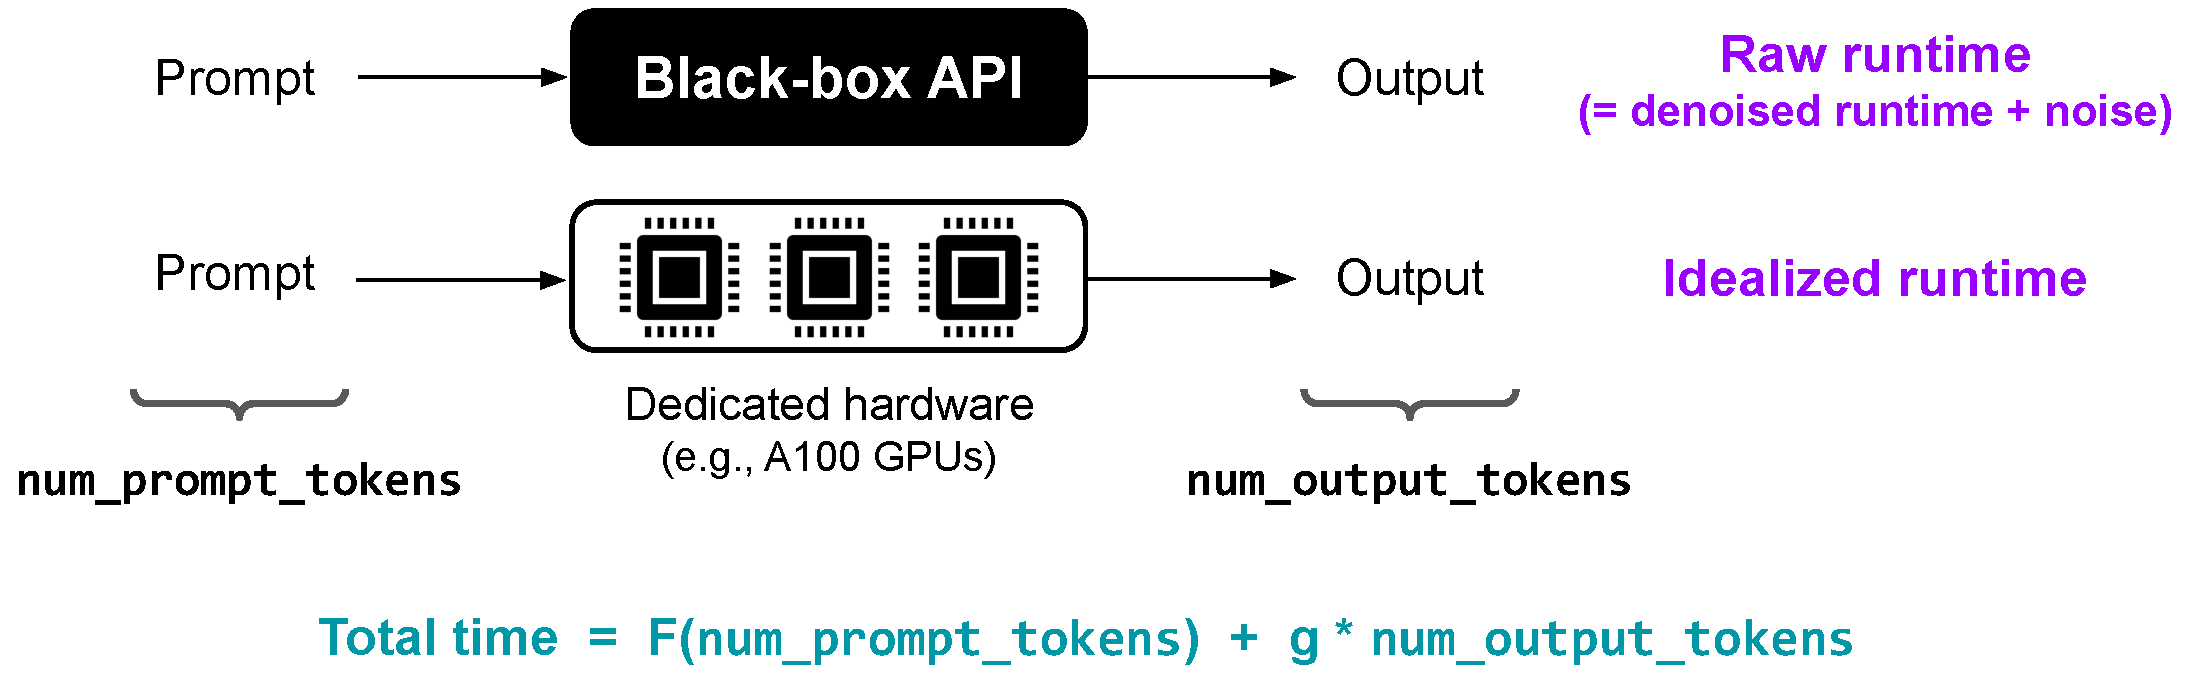
\includegraphics[width=0.75\textwidth]{figures/metrics_efficiency_v3.pdf}
  \caption{\textbf{Inference Efficiency Metrics.} A demonstration of how we measure inference efficiency. We compute two metrics: denoised inference runtime and idealized inference runtime. $F$ returns the runtime of encoding a prompt of given size, and $g$ is the runtime of generating each additional output token for the given model.}
  \label{fig:metrics-efficiency}
\end{figure}

These are unfortunately not \emph{fundamental} to the model itself, and consequently do not allow us to compare models on a level footing, which is the objective of this work. To be able to compare models more fairly, we designed two metrics:
\begin{itemize}
\item \textbf{Denoised inference runtime.} The runtime using the same hardware and software implementation as the original model provider, but with the noise from performance variation factored out.
\item \textbf{Idealized inference runtime.} The runtime using uniform \emph{optimized} hardware and software implementation, allowing for the inference efficiency of models to be directly compared against each other.
\end{itemize}

We present both of these metrics since we believe both are important: denoised runtimes give us an estimate for how long queries will take for end users using deployed interfaces such as OpenAI's API in the \emph{best case}, while idealized runtimes allow models to be more fairly compared and can be used to understand efficiency-capability tradeoffs. 
We present denoised runtimes for every model, and idealized runtimes for all models with publicly available model architecture information.
In practice, we measure idealized runtimes on NVIDIA A100 GPUs using Megatron~\citep{shoeybi2019megatron}, since we believe these are optimized hardware and software stacks (at the time of writing) with features like model parallelism that are needed to serve large LMs.
\reffig{metrics-efficiency} shows a visual comparison between these different inference runtime metrics, and also briefly explains how the denoised and idealized runtime metrics can be estimated. 

We can also derive idealized energy and idealized emitted CO$_2$ metrics from the idealized runtime, since we control the hardware on which the idealized runtimes are estimated.
Note that this cannot be done for the denoised runtimes since we do not know the hardware used by the model provider.